\documentclass[tikz,border=8pt]{standalone}
% Shared look for every TikZ diagram. Load with \input{../../tools/tikz-style.tex}
\usepackage[T1]{fontenc}
\usepackage{lmodern}
\renewcommand{\sfdefault}{lmr}  % diagrams use the same serif as the text
\usetikzlibrary{arrows.meta, positioning, shapes.geometric, calc, fit, backgrounds}
\definecolor{cblue}{HTML}{4C78A8}
\definecolor{corange}{HTML}{F58518}
\definecolor{cgreen}{HTML}{54A24B}
\definecolor{cred}{HTML}{E45756}
\definecolor{cpurple}{HTML}{B279A2}
\definecolor{cgrey}{HTML}{6B6B6B}
\tikzset{
  every picture/.style={font=\sffamily, line width=1.2pt},
  box/.style={draw=#1, fill=#1!12, rounded corners=4pt, align=center, inner sep=7pt, minimum height=1.1cm},
  box/.default=cgrey,
  arrow/.style={-{Stealth[length=3mm]}, draw=cgrey, line width=1.4pt},
  title/.style={font=\sffamily\bfseries\Large},
  note/.style={font=\sffamily\small, text=cgrey, align=center},
}
\AtBeginDocument{\hyphenpenalty=10000 \exhyphenpenalty=10000}

\begin{document}
% Section 3: the counting methods on the vocabulary (mat, cat, rat). One-hot: one row per word; bag of words: one
% row of counts per sentence. Neither says that two words are alike.
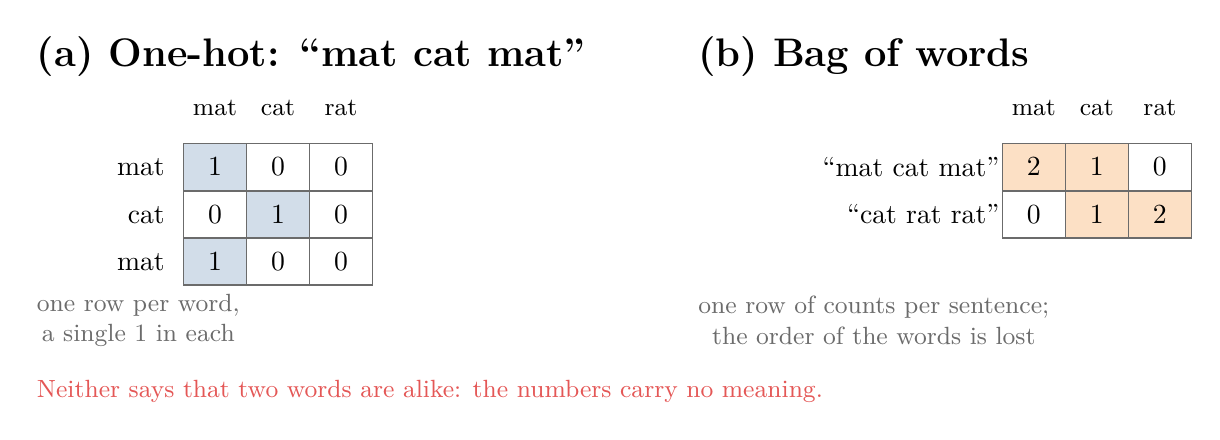
\begin{tikzpicture}[c/.style={draw=cgrey, minimum width=0.8cm, minimum height=0.6cm, font=\sffamily, line width=0.6pt},
                    one/.style={c, fill=cblue!25}, cnt/.style={c, fill=corange!25}]
  \node[title, anchor=west] at (-1.6, 1.4) {(a) One-hot: ``mat cat mat''};
  \foreach \v [count=\i] in {mat, cat, rat} \node[font=\sffamily\small] at (0.8*\i, 0.75) {\v};
  \foreach \w/\a/\b/\c [count=\r] in {mat/1/0/0, cat/0/1/0, mat/1/0/0} {
    \node[anchor=east, font=\sffamily] at (0.3, -0.6*\r + 0.6) {\w};
    \foreach \v [count=\k] in {\a, \b, \c} {\ifnum\v=1 \node[one] at (0.8*\k, -0.6*\r + 0.6) {1}; \else \node[c] at (0.8*\k, -0.6*\r + 0.6) {0}; \fi}
  }
  \node[note, anchor=west] at (-1.6, -1.95) {one row per word,\\a single 1 in each};
  \node[title, anchor=west] at (6.8, 1.4) {(b) Bag of words};
  \foreach \v [count=\i] in {mat, cat, rat} \node[font=\sffamily\small] at (10.4 + 0.8*\i, 0.75) {\v};
  \foreach \s/\a/\b/\c [count=\r] in {{mat cat mat}/2/1/0, {cat rat rat}/0/1/2} {
    \node[anchor=east, font=\sffamily] at (10.9, -0.6*\r + 0.6) {``\s''};
    \foreach \v [count=\k] in {\a, \b, \c} {\ifnum\v>0 \node[cnt] at (10.4 + 0.8*\k, -0.6*\r + 0.6) {\v}; \else \node[c] at (10.4 + 0.8*\k, -0.6*\r + 0.6) {0}; \fi}
  }
  \node[note, anchor=west] at (6.8, -1.95) {one row of counts per sentence;\\the order of the words is lost};
  \node[note, anchor=west, text=cred] at (-1.6, -2.85) {Neither says that two words are alike: the numbers carry no meaning.};
\end{tikzpicture}
\end{document}
